\section{Results} \label{sec:Phase_II_results}

The expected Phase-2 \mgg distributions are shown in Figure~\ref{fig:prefit} for the semi-leptonic \wwgg final state, and one tau \ttgg final state. 

\begin{figure}[!htbp]
    \setcounter{subfigure}{0}
    \centering
    \subfloat[Semi-leptonic final state]{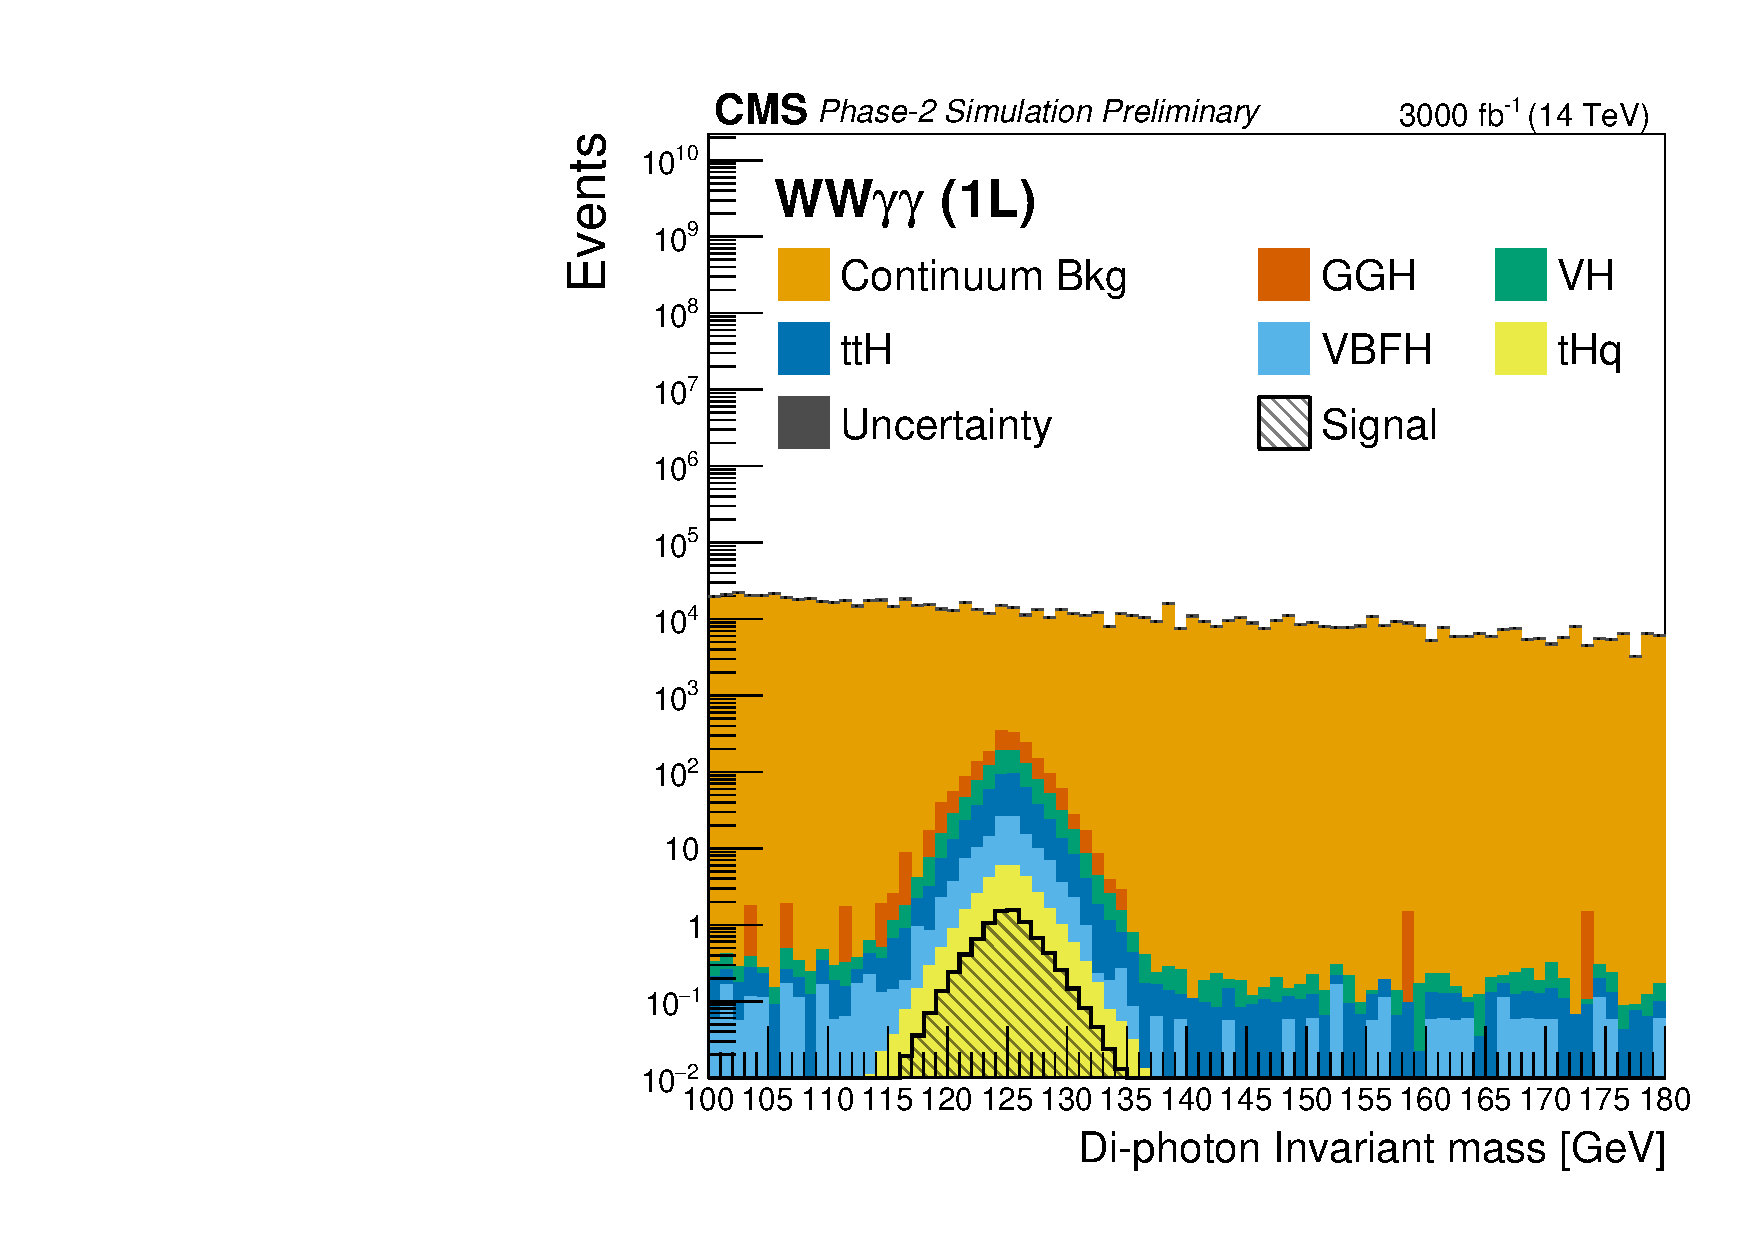
\includegraphics[width=0.45\textwidth]{Sections/Phase_II_HH/images/Results/CombineInputs/WWgg_1L_prefit_log_unblinded_False_HL.pdf}}
    \qquad
    \subfloat[One tau final state]{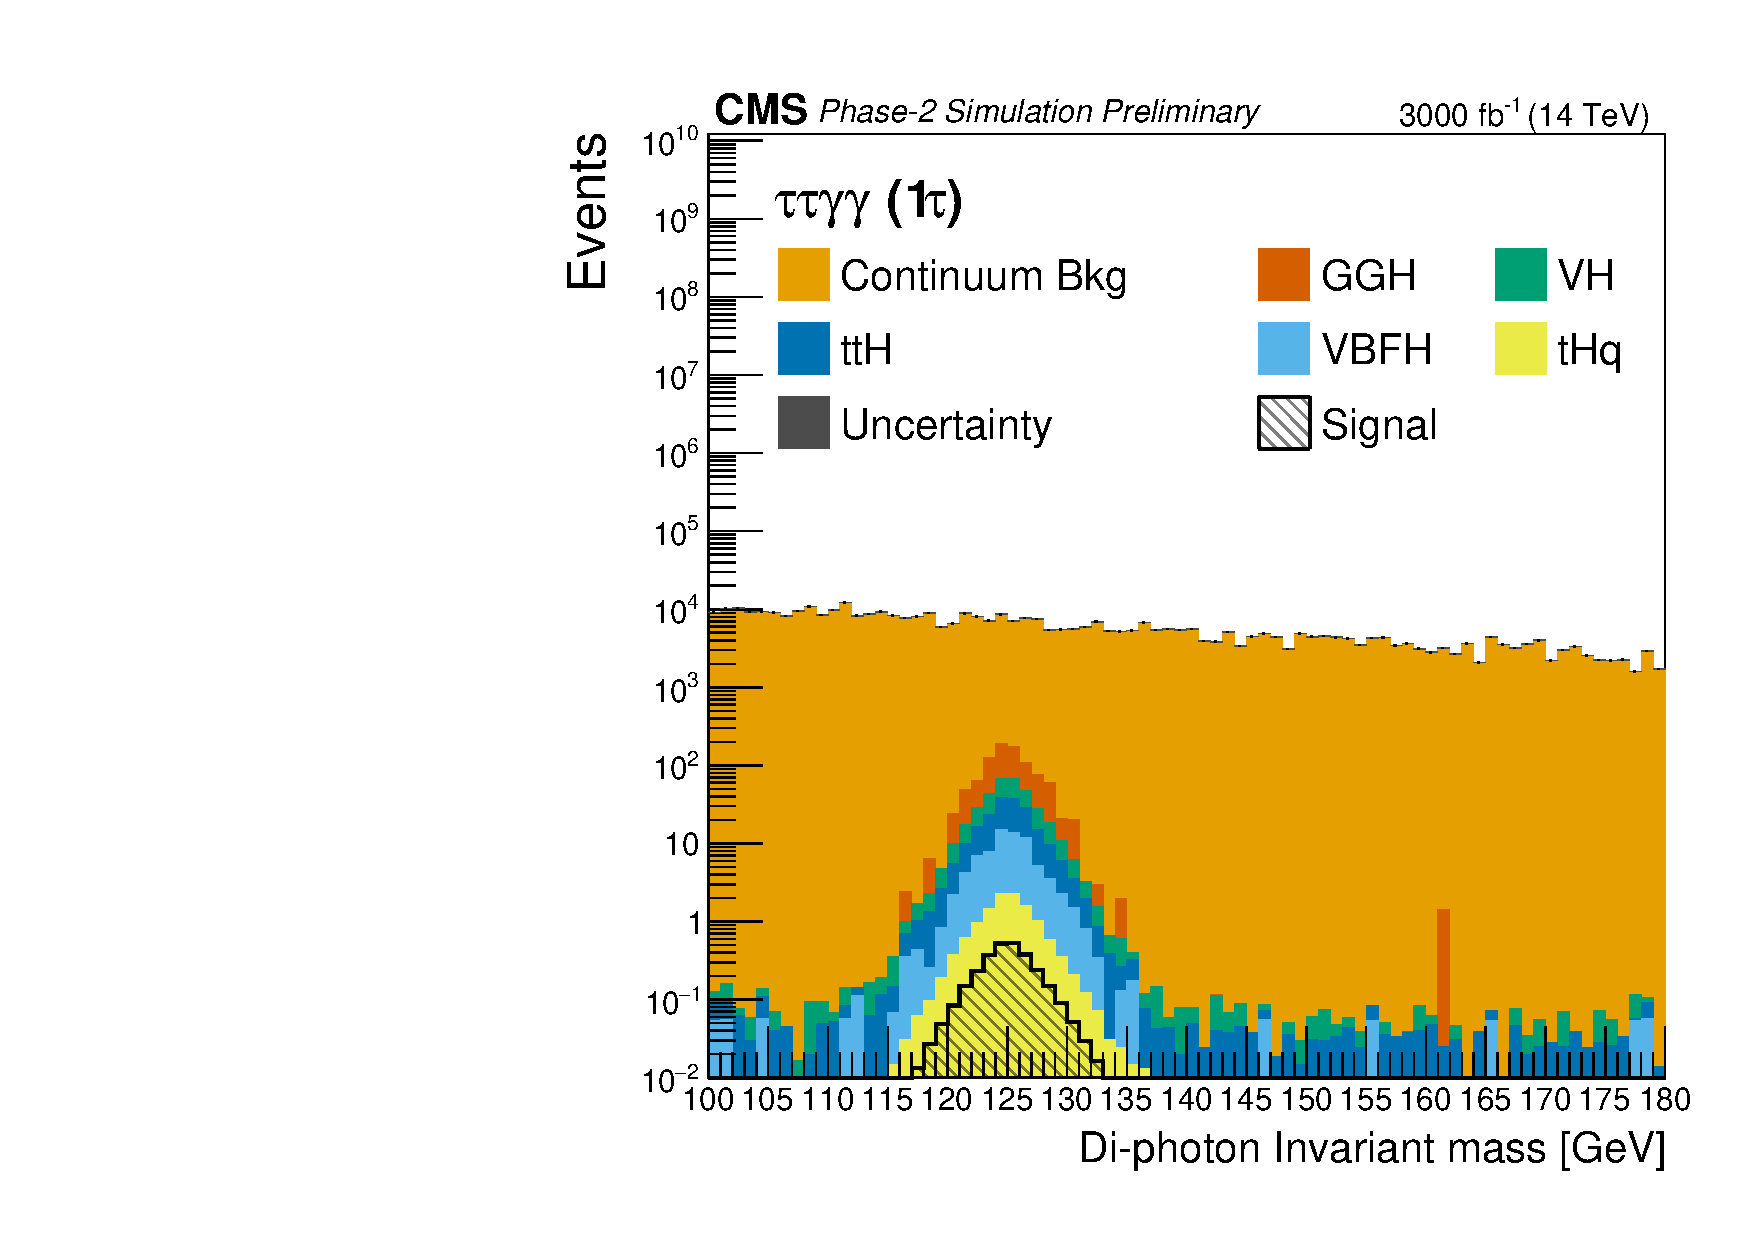
\includegraphics[width=0.45\textwidth]{Sections/Phase_II_HH/images/Results/CombineInputs/ttgg_prefit_log_unblinded_False_HL.pdf}}
    \caption{$m_{\gamma\gamma}$ distributions in the \wwgg, Semi-leptonic (left) and \ttgg, 1$\tau$ (right) final states.}
    \label{fig:prefit}
\end{figure}

Given the presence of high fluctuations in the \mgg distribution of the continuum background across different categories, a falling exponential function is fit to the continuum background templates and used as the final background template for each category. After applying this exponential fit, and a gaussian fit to each HH and H template, the diphoton invariant mass distributions for the Semi-leptonic final state in its most sensitive category, the single fully-leptonic category and in the single 2 $\tau$ final state category are shown in Figure \ref{fig:final_plots}, where signal HH and single Higgs templates are modelled as Gaussian functions fit to the diphoton mass distributions, and the continuum background is modelled by exponential functions. The (pseudo-)data are generated according to the fitted signal, single Higgs and continuum background contributions.  

\begin{figure}[!htbp]
    \setcounter{subfigure}{0}
    \centering
    \subfloat[Semi-leptonic final state, Category 4]{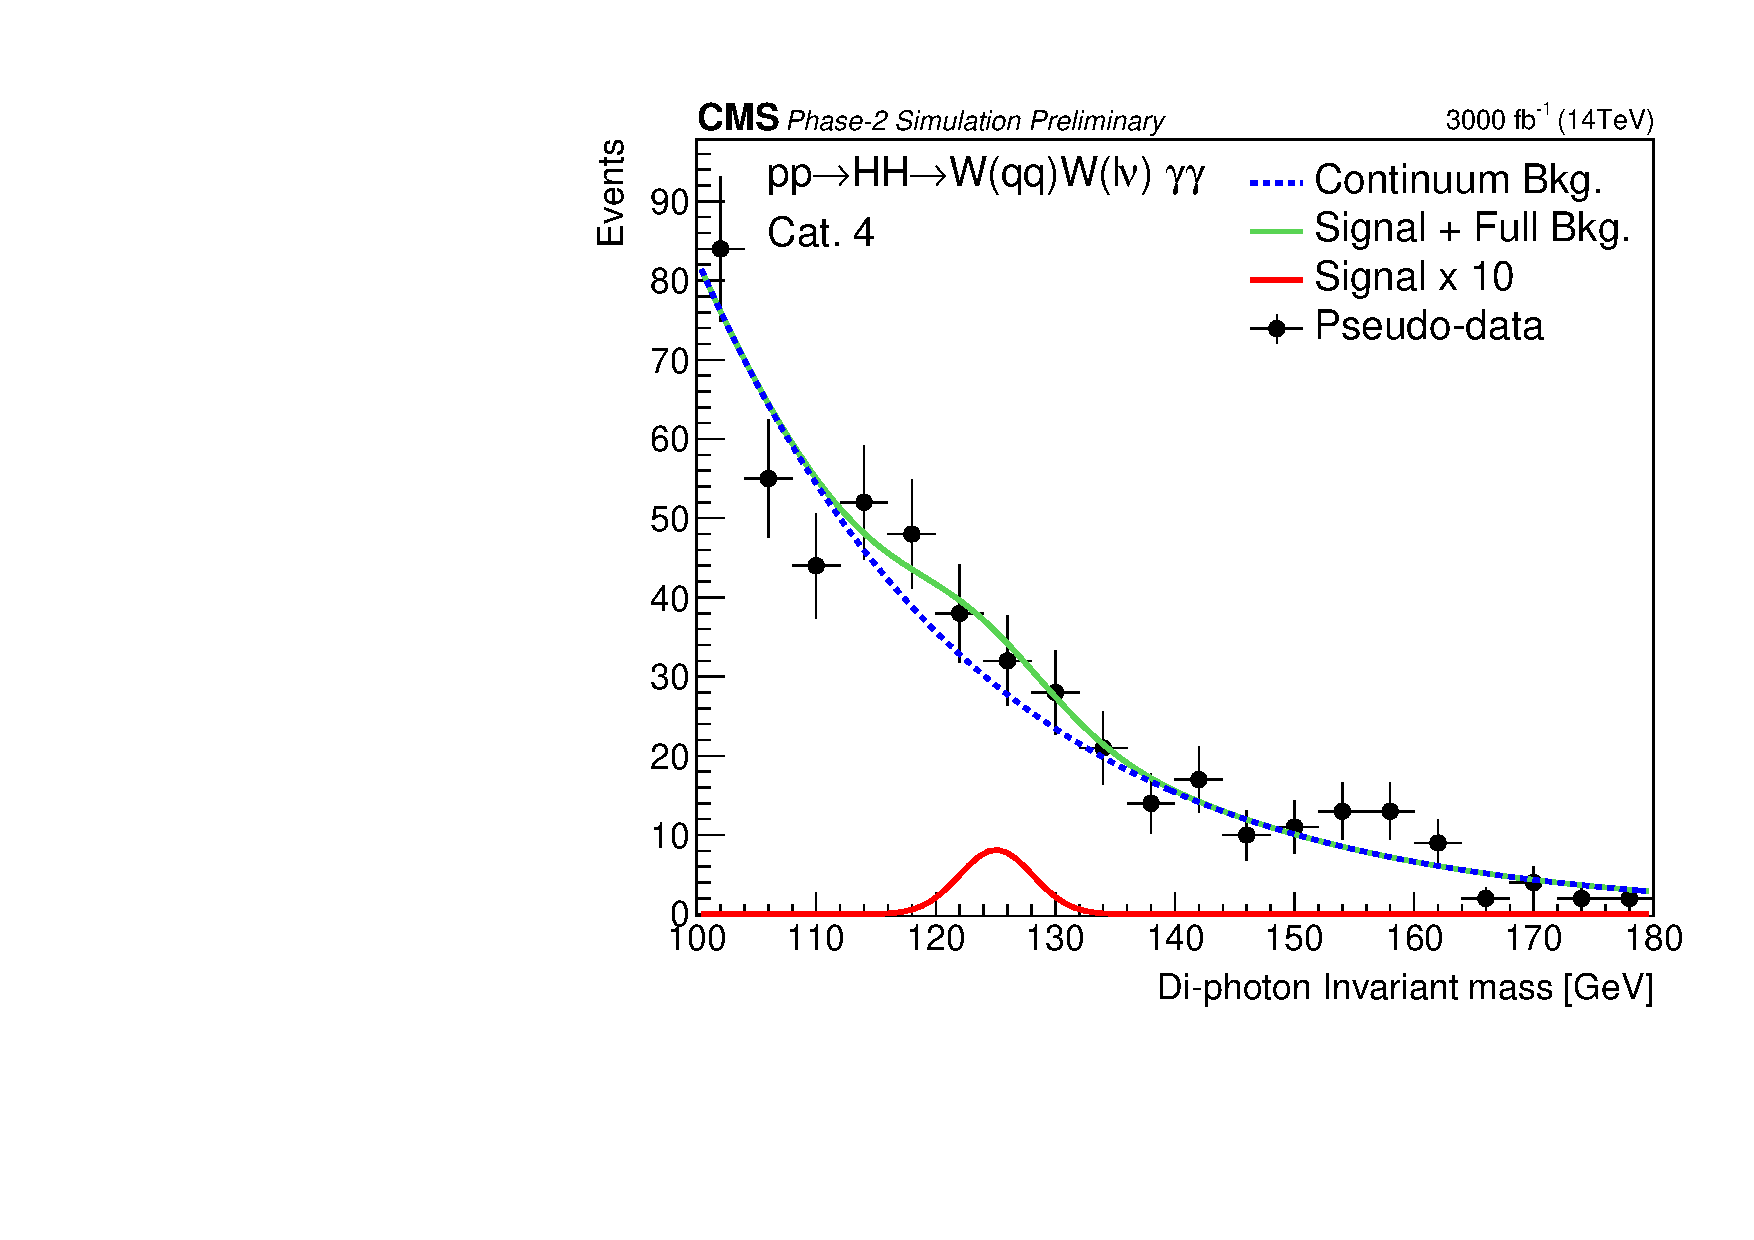
\includegraphics[width=0.45\textwidth]{Sections/Phase_II_HH/images/Results/Inv_mass_gghasOneL_DNN_4_HL_FIT.pdf}}
    \qquad
    \subfloat[Fully-leptonic final state]{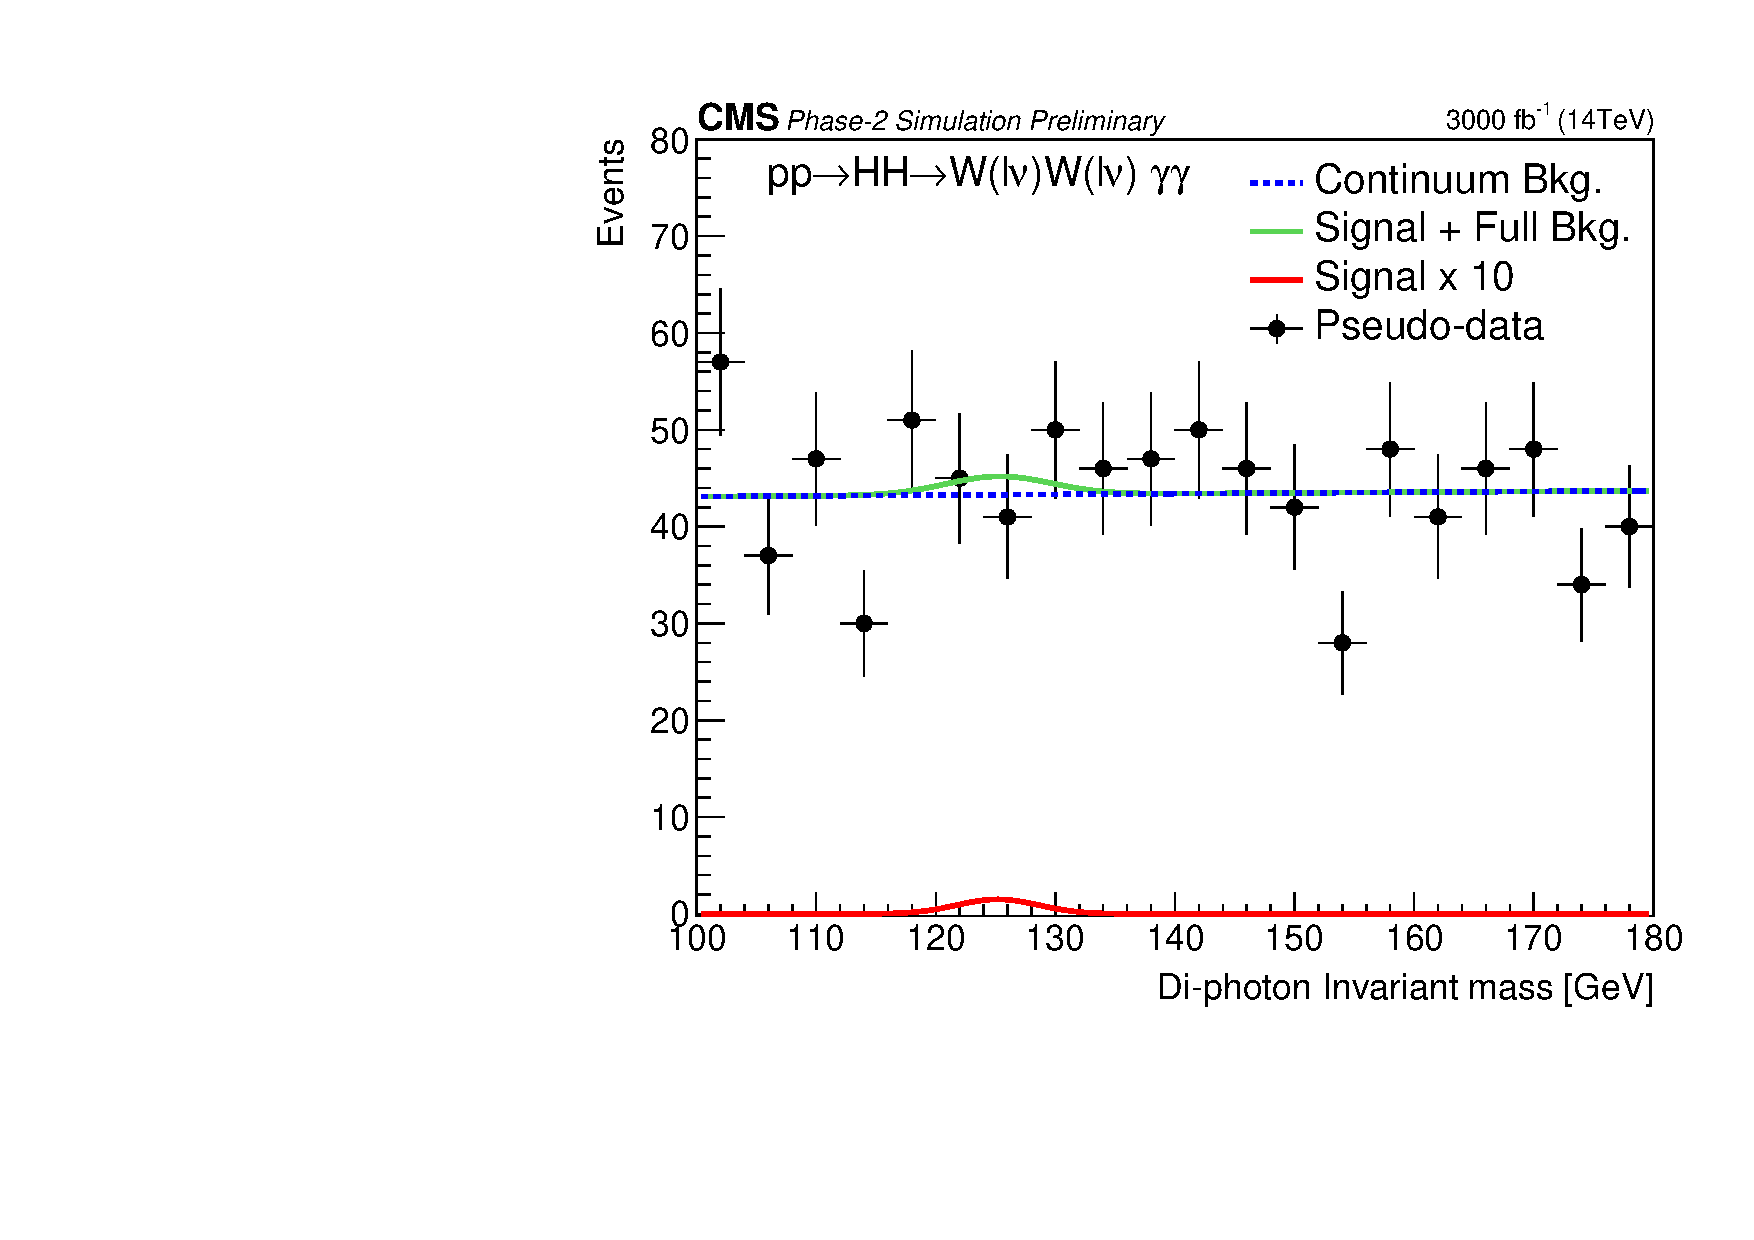
\includegraphics[width=0.45\textwidth]{Sections/Phase_II_HH/images/Results/Inv_mass_gghasTwoL_HL_FIT.pdf}}
    \qquad
    \subfloat[Two taus final state]{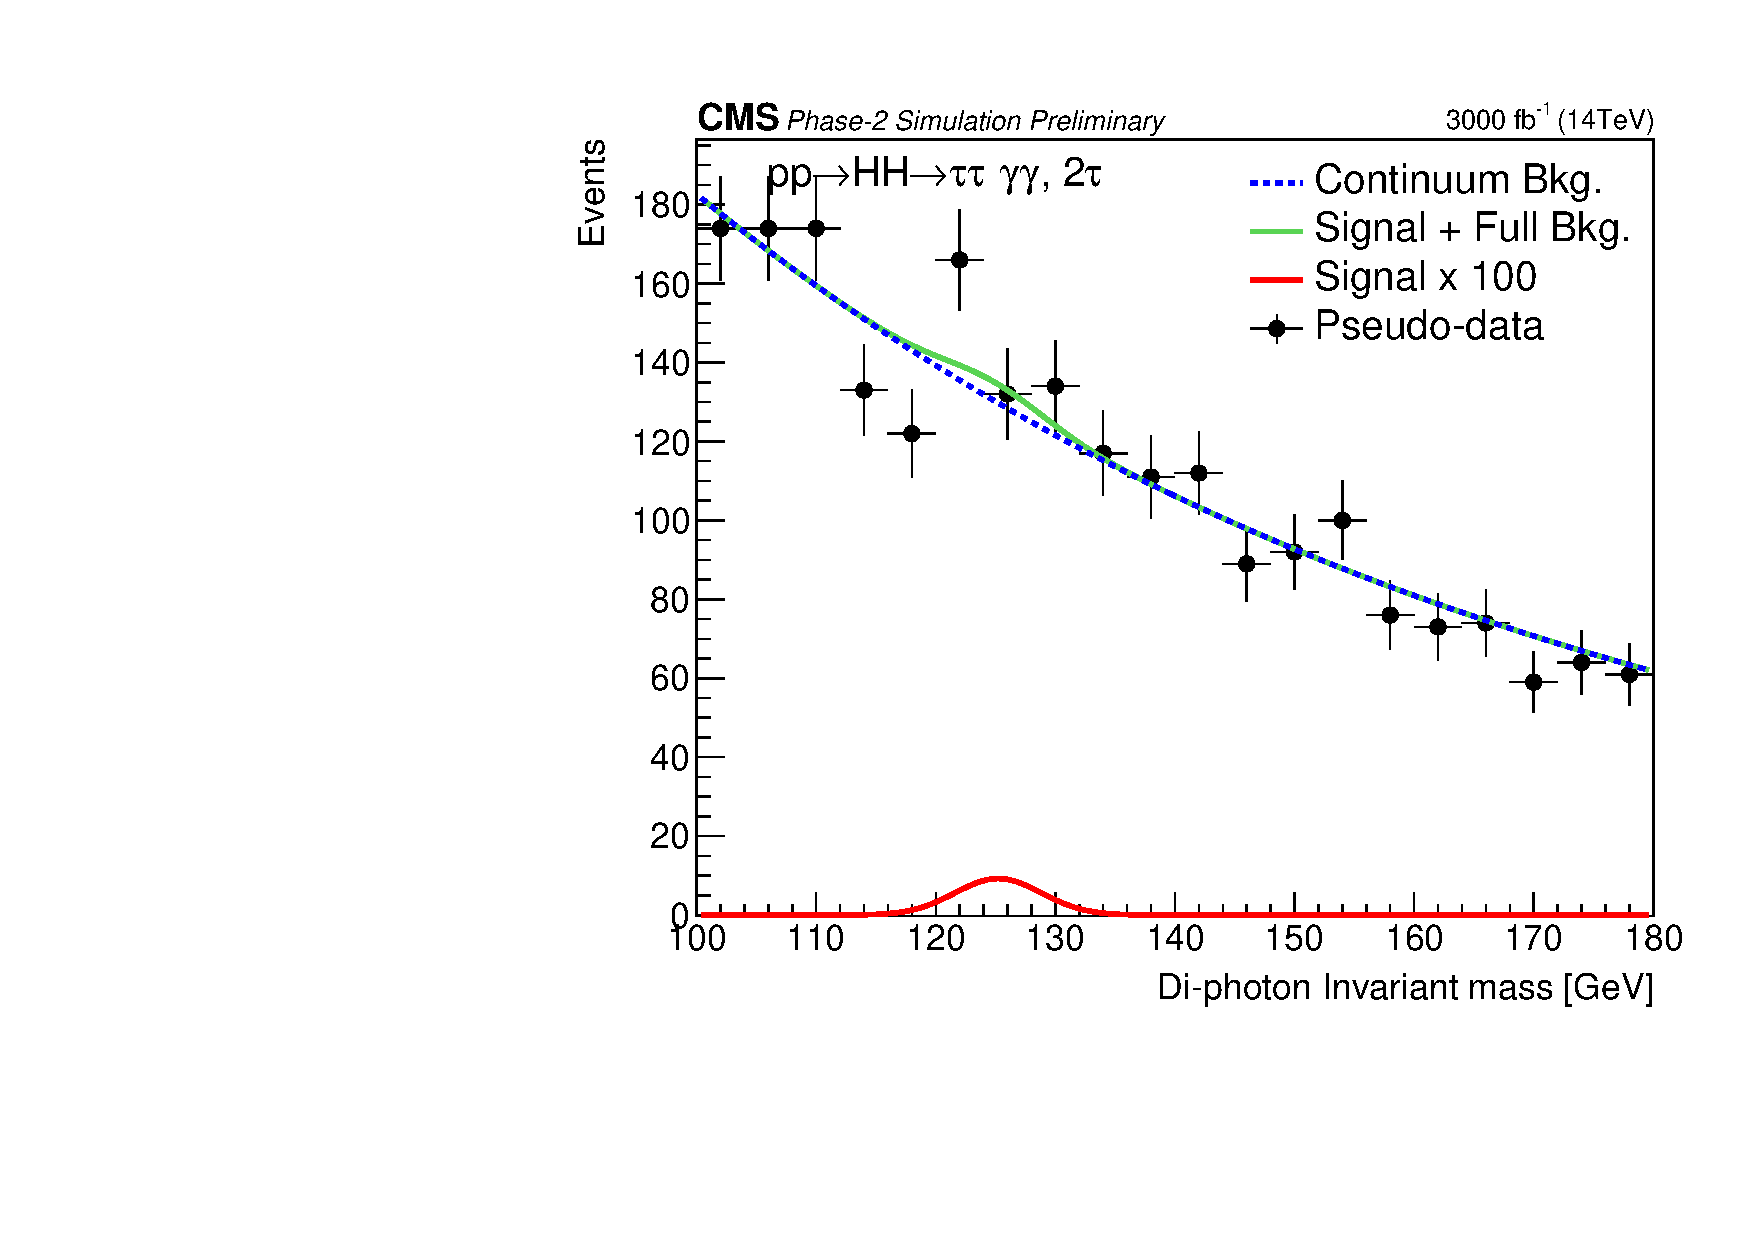
\includegraphics[width=0.45\textwidth]{Sections/Phase_II_HH/images/Results/Mgg_c4_Zveto_HL_FIT.pdf}}
    \caption{$m_{\gamma\gamma}$ distributions in the \wwgg, Semi-leptonic (top left), Fully-leptonic (top right) and \ttgg, 2$\tau$s (bottom) final states.}
    \label{fig:final_plots}
\end{figure}

The expected signal significance is extracted by fitting the background-only \mgg template to the signal $+$ background template simultaneously in all categories, following a binned maximum likelihood
approach, with all systematic uncertainties treated as nuisance parameters with log-normal distributions. The correlations among different sources of uncertainties are taken into account while the different final states are considered as independent channels in the fit. 

The significance values obtained are shown in Table~\ref{tab:combinedSignificance} for the WW$\gamma\gamma$ and \ttgg final states along with their combination.

\begin{table}[h!]
  \centering
  \begin{tabular}{lc}
    \hline 
    Final State & Significance (stat+exp+theory) \\
\hline

    \wwgg & 0.21  \\ 
    \ttgg &  0.08 \\
   Combination &  0.22 \\ 

    \hline
   \end{tabular}
    \caption{
        Expected HL-LHC significances ($\sigma$) results of the WW$\gamma\gamma$ and \ttgg processes with their combination.
        }
    \label{tab:combinedSignificance}
\end{table}

A combined significance of 0.22$\sigma$ is extracted, combining the \wwgg and \ttgg categories. 